\documentclass[../notes.tex]{subfiles}

\pagestyle{main}
\renewcommand{\chaptermark}[1]{\markboth{\chaptername\ \thechapter\ (#1)}{}}
\setcounter{chapter}{7}

\begin{document}




\chapter{Exterior Algebra}
\section{Linear Algebra Review and Rational Canonical Form}
\begin{itemize}
    \item \marginnote{2/20:}Nori's change of heart.
    \begin{itemize}
        \item We've all seen linear algebra; thus, we'll speedrun it and then do exterior algebra and determinants. That's where we'll finish.
    \end{itemize}
    \item The following is part 1 of a linear algebra course.
    \item Let $F$ be a field.
    \item \textbf{Vector space}: An $F$-module.
    \item \textbf{Linearly independent} (subset $S\subset V$): Same definition we're familiar with.
    \item \textbf{Spanning} (subset $S\subset V$): A subset $S$ of $V$ that is a set of generators of $V$.
    \item $S$ is a \textbf{basis} implies that $S$ generates $V$ and is linearly independent.
    \item Every linearly independent subset of $V$ can be extended to a basis.
    \item Every spanning set $S$ contains a basis.
    \begin{itemize}
        \item Any maximal linearly independent subset of $S$ is a basis.
    \end{itemize}
    \item $S_1,S_2$ are bases for $V$ implies that $|S_1|=|S_2|$.
    \begin{itemize}
        \item The replacement theorem in \textcite{bib:DummitFoote} is a good way to prove this.
    \end{itemize}
    \item We are now done with part 1; this is part 2 of a linear algebra course.
    \item Let $T:V\to V$ be a linear transformation.
    \item Let $A$ be a ring. What is an $A[X]$-module $M$?
    \begin{itemize}
        \item It is an abelian group $(M,+)$ and a ring homomorphism $\rho:A[X]\to\End(M,+)$.
        \item Since $A\hookrightarrow A[X]$, $\rho|_A$ turns $M$ into an $A$-module.
        \item Since $aX=Xa$, $\rho(a)\rho(X)=\rho(X)\rho(a)$.
        \item But since we consider $M$ to be a module, we write $a:=\rho(a)$: Thus, $a\rho(X)m=\rho(X)am$ for all $m\in M$.
        \item Note that $\rho(X)\in\End_A(M)$ (which is the set of all $A$-module endomorphisms).
        \item Additionally, $\rho(X):M\to M$ is an $A$-module homomorphism.
    \end{itemize}
    \item Put $\rho(X)=T$. Thus, an $A[X]$-module is a pair $(M,T)$, where $M$ is an $A$-module and $T\in\End_A(M)$.
    \item Conversely, such $(M,T)$ gives rise to an $A[X]$-module with action
    \begin{equation*}
        \left( \sum_{n=0}^\ell a_nX^n \right)m = \sum_{n=0}^\ell a_nT^nm
    \end{equation*}
    \item Let $F$ be a field, and consider $(V,T)$ where $V$ is any $F$-vector space and $T:V\to V$ is a linear transformation.
    \begin{itemize}
        \item This induces a module over $F[X]$.
    \end{itemize}
    \item $V$ finite dimensional induces $\rho:F[X]\to\End_F(V)\cong M_n(F)$ defined by $X\mapsto T$.
    \begin{figure}[H]
        \centering
        \begin{tikzpicture}[xscale=2,yscale=1.6]
            \small
            \node (R)  at (0,1) {$F[X]$};
            \node (DR) at (0,0) {$F[X]/(f)$};
            \node (S)  at (1,1) {$\End_F(V)$};
    
            \footnotesize
            \draw [->]           (R)  --                                     (DR);
            \draw [right hook->] (DR) -- node[above left=-2pt]{$\bar{\rho}$} (S);
            \draw [->]           (R)  -- node[above]          {$\rho$}       (S);
        \end{tikzpicture}
        \caption{$F[X]$-module actions.}
        \label{fig:fXmodAction}
    \end{figure}
    \begin{itemize}
        \item $\rho(X)=T$ and $\rho(c)=c$ for all $c\in F$.
        \item $\ker(\rho)=(f)$ for some monic polynomial $f$ of degree $d\leq n^2$.
        \item We have the constraint on the degree of $f$ by the isomorphism from Lecture 3.1.
    \end{itemize}
    \item \textbf{Minimal polynomial} (of $T$): The polynomial $f$ that generates $\ker(\rho)$.
    \begin{itemize}
        \item In particular, $V$ is a finitely generated torsion $F[X]$-module.
    \end{itemize}
    \item \textbf{Cyclic vector}: A vector $v\in V$ belonging to $(V,T)$ such that $v,Tv,T^2v,\dots$ spans $V$.
    \item Using cyclic vectors to compute the minimal polynomial.
    \begin{itemize}
        \item Assume $v,Tv,T^2v,\dots,T^{k-1}v$ are linearly independent, but $v,Tv,\dots,T^kv$ are not.
        \item Then
        \begin{equation*}
            T^kv = a_0v+a_1Tv+\cdots+a_{k-1}T^{k-1}v
        \end{equation*}
        where all $a_i\in F$ and not all $a_i=0$.
        \item Let $W=\gen{v,Tv,\dots,T^{k-1}v}$. It follows that $T^mk\in W$.
        \item Let
        \begin{equation*}
            g(X) = X^k-(a_{k-1}X^{k-1}+\cdots+a_1X+a_0)
        \end{equation*}
        Then $g(T)v=0$. This implies that $g$ is the minimal polynomial of $T$.
        \item It follows that $T^hg(T)v=0$. Thus, $g(T)T^hv=0$ for all $h$.
        \item Lastly, it follows that $g(T)w=0$ for all $w\in W$.
        \item Assume $v$ is a cyclic vector. Then $W=V$. It follows that $g(T)v=0$ for all $v\in V$.
        \item The original assumption posits that no polynomial of degree less than or equal to $k-1$ can annihilate $v$.
    \end{itemize}
    \item Consider $V=F[X]/(f)$. Let $\deg(f)=d$, let $T:V\to V$, and let $T$ be the "multiply by $X$" linear transformation. It follows that if $v_i=\overline{X^{i-1}}$ ($i=1,\dots,d$), then
    \begin{equation*}
        Tv_i = v_{i+1}
    \end{equation*}
    for $i=1,\dots,d-1$ and
    \begin{equation*}
        Tv_d = -(a_0v_1+a_1v_2+\cdots+a_{d-1}v_d)
    \end{equation*}
    \begin{itemize}
        \item If $d=3$, then we have
        \begin{equation*}
            M(T) =
            \begin{pmatrix}
                0 & 0 & -a_0\\
                1 & 0 & -a_1\\
                0 & 1 & -a_2\\
            \end{pmatrix}
        \end{equation*}
        \item The above matrix is called the \textbf{companion matrix} of $f$, for $f$ monic of degree 3.
    \end{itemize}
    \item \textbf{Rational canonical form}: The form $(V,T)$ given by
    \begin{equation*}
        F[X]/(f_1)\oplus\cdots\oplus F[X]/(f_s)
    \end{equation*}
    where $f_2\mid f_1$, \dots, $f_s\mid f_{s-1}$ and $\deg(f_s)>0$.
    \begin{itemize}
        \item When $V=0$, then $s=0$. In this case, $f_1$ is the minimal polynomial of $T$.
        \item The form consisting of a block diagonal matrix of companion matrices.
    \end{itemize}
    \item \textbf{Jordan canonical form}:
    \begin{itemize}
        \item Has to do with $p$-primary components!
    \end{itemize}
    \item There's one more canonical form, too.
    \item Since no one knows what canonical forms are and we very much need them for what Nori was planning to do, Nori will change his plans. No tensors in the last week, either.
    \item $p$-primary components: When $p=X-a$, $a\in F$.
    \item $(V,T)$ is \textbf{$\bm{p}$-primary} if there exists an $n$ such that $(T-a)^nv=0$ for all $v\in V$.
    \item $1_V:V\to V$ is the identity.
    \item $a\cdot 1_V=a_V:V\to V$.
    \item $(T-a_v)^n=0\in\End_F(V)$.
    \item We're now doing generalized eigenspaces ?? lol.
    \item The $p$-primary component is as the generalized $a$-eigenspace.
    \begin{itemize}
        \item $(T-a)v=0$, i.e., $Tv=av$ is the $a$-eigenspace; the eigenspaces are components of the generalized eigenspaces.
    \end{itemize}
    \item Let $V=F[X]/(X-a)^n$. Let $v_1=1$, $v_2=\overline{X-a}$, \dots, $v_n=\overline{(X-a)^{n-1}}$.
    \begin{itemize}
        \item We know that $X(X-a)^r=(X-a+a)(X-a)^r=(X-a)^{r+1}+a(X-a)^r$.
        \item Nori writes Jordan blocks as
        \begin{equation*}
            \begin{pmatrix}
                a & 0 & 0 & 0\\
                1 & a & 0 & 0\\
                0 & 1 & a & 0\\
                0 & 0 & 1 & a\\
            \end{pmatrix}
        \end{equation*}
        not with 1's in the superdiagonal.
        \begin{itemize}
            \item Thus, the \emph{last} generalized eigenvector is an eigenvector here, instead of the \emph{first}.
        \end{itemize}
    \end{itemize}
\end{itemize}



\section{Office Hours (Nori)}
\begin{itemize}
    \item Midterm: We never covered the universal property of a quotient in class, did we?
    \begin{itemize}
        \item That's the special lemma from last office hours.
    \end{itemize}
    \item PSet 7: 7.3 and 7.4 typos.
    \item Wednesday lecture?
    \begin{itemize}
        \item Seventh week summary will suffice.
    \end{itemize}
    \item What do you need us to know about the rational canonical form? Should I still read \textcite{bib:DummitFoote}, Section 12.2 or is that no longer necessary?
    \begin{itemize}
        \item Nori will probably push ahead with 12.2. Thus I should read it. He's not sure what he'll do beyond that, though, since he doesn't want to jam tensors into the last week.
        \item I will need tensor products for representation theory, regardless, so if I want to take it, I should self-study it.
        \item No chance tensor products will be covered next quarter.
        \item Serre is a terrific mathematician whose wife is a super chemist, and that's why he wrote his book on representation theory (and wrote it in a less terse manner than usual).
        \item No tensors means no exterior algebra, too.
        \item Nori hasn't read any of \textcite{bib:DummitFoote}.
        \item The transfer theory of groups arises in a later chapter, and that's important for representation theory, though.
    \end{itemize}
    \item Nori doesn't think any teacher pays attention to what courses are supposed to cover as stated in the course catalog.
    \begin{itemize}
        \item We will never do modules, multilinear and quadratic forms.
        \item $p$-adic field and Galois theory.
        \item Nori thinks the proof of Theorem \ref{trm:12.4} is very difficult to follow for a first-timer.
        \item Solvable groups were supposed to be a MATH 25700 topic, but got cut because of 9-week quarters.
        \item Syclotomic fields have applications to the representation theory of finite groups; there are theorems of representation theory that you need syclotomic fields to prove.
        \item Emil Artin: Galois Theory is worth looking up.
        \item Gauss and constructions of 17-gons also needs syclotomic fields.
    \end{itemize}
\end{itemize}



\section{Office Hours (Nori)}
\begin{itemize}
    \item \marginnote{2/21:}Lecture 6.1: Proposition proof?
    \item Lecture 6.1: $(2)\subsetneq\Z$ example?
    \item Lecture 6.1: The end of the theorem proof.
    \item Lecture 6.2: Does the first theorem you proved not appear in the book until Chapter 12?
    \item Lecture 6.2: What is $A$ in the proof?
    \item Resources for the proofs in Week 6?
    \item Lecture 7.1: Quotient stuff.
    \item Lecture 7.2: Why does $\Ann(v)=(p^k)$, why not just $(p^k)\subset\Ann(v)$? Additionally, how does $p^kw'=0$ imply that $p^k\in\Ann(w)$?
    \begin{itemize}
        \item $R$ is a PID!
        \item $\Ann(w)$ should be $\Ann(w')$ in the centered line.
        \item We don't need to know the theorem from the book for a while (second year of graduate school at least).
        \item It's good to know the proofs from class just for going forward in math, but we probably will not be asked to reproduce them on an exam.
    \end{itemize}
    \item Lecture 7.3: RCF proof?
    \begin{itemize}
        \item It's not $m_i,1$, it's $m_{i,1}$!
        \item Rewrite the proof when I'm awake enough to understand it.
    \end{itemize}
\end{itemize}



\section{Noncommutative Polynomial Rings}
\begin{itemize}
    \item \marginnote{2/22:}Adjusted syllabus for those of us who haven't seen block matrices.
    \begin{itemize}
        \item We're not gonna cover all of the stuff in Sections 12.2-12.3.
        \item We'll define determinants via exterior algebras and use them to prove the Cayley-Hamilton theorem.
    \end{itemize}
    \item Notation for today:
    \begin{itemize}
        \item We fix $R$ a commutative ring.
        \item Any other ring considered is potentially noncommutative.
        \item $c$ denotes an element of $R$.
    \end{itemize}
    \item \textbf{$\bm{R}$-algebra}: A pair $(A,\phi)$ where $A$ is a ring and $\phi:R\to A$ is a ring homomorphism such that
    \begin{equation*}
        \phi(c)a = a\phi(c)
    \end{equation*}
    for all $a\in A$ and $c\in R$.
    \begin{itemize}
        \item I.e., we have commutativity with the "integers."
        \item Notation: We suppress the letter $\phi$.
        \begin{itemize}
            \item Justification: $A$ can be considered an $R$-module in a natural manner, so we can use the standard notation $c\cdot a$ in place of $\phi(c)\cdot a$ because we can think of $\phi$ as the action of $R$ on $A$.
        \end{itemize}
        \item $R$-algebras are automatically $R$-modules.
        \item $\phi(R)$ is a subring of $A$ (and, specifically, the center of $A$).
    \end{itemize}
    \item Now we get into noncommutative polynomial rings.
    \begin{itemize}
        \item We've defined polynomial rings on one variable, and on multiple variables by induction.
        \item There, the variables commuted. However, they need not! We can construct rings such that $XY\neq YX$.
    \end{itemize}
    \item Consider the ring consisting of $n$ potentially noncommutative variables over the coefficients in $R$.
    \begin{itemize}
        \item Essentially, we postulate that $1,X_1,X_2,\dots,X_n$ are in the ring and consider the set of everything that can be generated from these elements via addition, multiplication, and the action of $R$.
        \item Thus, things like $X_iX_j$ exist. Note that there are $n^2$ of these. Things like $X_iX_jX_k$ also exist (and there are $n^3$ of these).
    \end{itemize}
    \item Polynomials will be of the form
    \begin{equation*}
        c_0+\sum_{i=1}^nc_iX_i+\sum_{\substack{1\leq i\leq n\\1\leq j\leq n}}c_{i,j}X_iX_j+\cdots
    \end{equation*}
    \begin{itemize}
        \item This polynomial has degree at most $n$.
        \begin{itemize}
            \item Really?? How does Nori define degree? This would appear to be a break from the convention introduced in Section 9.1.
        \end{itemize}
        \item Note that since this is not a \textbf{noncommutative power series ring}, we assume that all polynomials have a finite degree.
    \end{itemize}
    \item \textbf{Free $\bm{R}$-algebra} (on the set $S$): The free $R$-module on the set $\{1\}\sqcup S\sqcup S\times S\sqcup S\times S\times S\sqcup\cdots$. \emph{Denoted by} $\bm{F_R(S)}$.
    \begin{itemize}
        \item Elements of the set include $1$, $X_s$ for all $s\in S$, $X_sX_t$ for all $s,t\in S$, etc.
        \item Multiplication is still associative: $(X_{s_1}X_{s_2})(X_{t_1}X_{t_2}X_{t_3})=X_{s_1}X_{s_2}X_{t_1}X_{t_2}X_{t_3}$.
        \item We still have commutativity for coefficients (i.e., $X_sc=cX_s$ for all $c\in R$ and $s\in S$) since $F_R(S)$ is an $R$-algebra.
        \begin{itemize}
            \item Did Nori qualify this?? Did he say that we do not write the $c_i$'s at the front any more?
        \end{itemize}
    \end{itemize}
    \item \textbf{$\bm{R}$-algebra homomorphism}: A function $h:A\to B$, where $A,B$ are $R$-algebras, such that\dots
    \begin{enumerate}[label={(\roman*)}]
        \item $h$ is a ring homomorphism;
        \item $h(c)=c$ for all $c\in R$.
    \end{enumerate}
    \begin{figure}[h!]
        \centering
        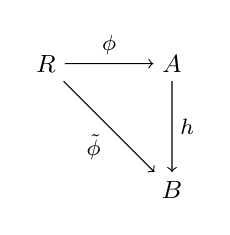
\begin{tikzpicture}[scale=1.6]
            \small
            \node (R) at (0,1) {$R$};
            \node (A) at (1,1) {$A$};
            \node (B) at (1,0) {$B$};
    
            \footnotesize
            \draw [->] (R) -- node[above]         {$\phi$}         (A);
            \draw [->] (A) -- node[right]         {$h$}            (B);
            \draw [->] (R) -- node[below left]{$\tilde{\phi}$} (B);
        \end{tikzpicture}
        \caption{Visualizing $R$-algebra homomorphisms.}
        \label{fig:RalgHom}
    \end{figure}
    \begin{itemize}
        \item For clarity: If we momentarily drop our convention of suppressing $\phi$, (ii) means $h(\phi(c))=\tilde{\phi}(c)$ for all $c\in R$.
        \item Alternate form of (ii): $h$ is an $R$-module homomorphism.
        \begin{itemize}
            \item This expresses the idea that the action of elements $c\in R$ on $A$ is preserved under $h$, i.e., if $c\cdot a=ca$, then $ch(a)=c\cdot h(a)=h(c)\cdot h(a)=h(c\cdot a)=h(ca)$.
        \end{itemize}
    \end{itemize}
    \item Universal property of $F_R(S)$: Consider $i:S\to F_R(S)$ defined by $i(s)=X_s$. It is a map of sets since $S$ has no additional structure. Given an $R$-algebra $A$ and function $j:S\to A$, there exists a unique $R$-algebra homomorphism $h:F_R(S)\to A$ such that the following diagram commutes, i.e., $h(i(s))=j(s)$ for all $s\in S$.
    \begin{figure}[H]
        \centering
        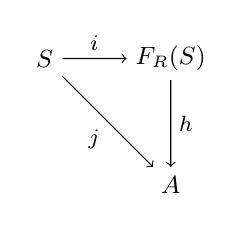
\begin{tikzpicture}[scale=1.6]
            \small
            \node (R) at (0,1) {$S$};
            \node (A) at (1,1) {$F_R(S)$};
            \node (B) at (1,0) {$A$};
    
            \footnotesize
            \draw [->] (R) -- node[above]     {$i$} (A);
            \draw [->] (A) -- node[right]     {$h$} (B);
            \draw [->] (R) -- node[below left]{$j$} (B);
        \end{tikzpicture}
        \caption{Universal property of $F_R(S)$.}
        \label{fig:univPropFRS}
    \end{figure}
    \item The principle of this universal property is the same as that of the universal property of polynomial rings. Seeing this:
    \begin{itemize}
        \item Since $i(s)=X_s$, the statement $h(i(s))=j(s)$ becomes $h(X_s)=j(s)$ for all $s\in S$.
        \item This combined with the fact that $h$ is an $R$-algebra homomorphism forces both existence and uniqueness for a reason symmetric to the proof of the universal property of polynomial rings in Lecture 1.2.
    \end{itemize}
    \item We now develop a related object that appears in Chapter 10 called a \textbf{tensor algebra}.
    \begin{itemize}
        \item A tensor algebra is very similar to a noncommutative polynomial ring.
    \end{itemize}
    \item \textbf{Tensor algebra} (of $M$): A pair $(A,\alpha)$, where $A$ an $R$-algebra and $\alpha:M\to A$ is an $R$-module homomorphism. \emph{Denoted by} $\bm{T(M)}$.
    \item Universal property of the tensor algebra $T(M)$: $T(M)$ is an $R$-algebra, $u:M\to T(M)$ is an $R$-module homomorphism such that for all pairs $(A,\alpha:M\to A)$, there exists a unique $R$-algebra homomorphism $f:T(M)\to A$ such that the following diagram commutes, i.e., $f\circ u=\alpha$.
    \begin{figure}[H]
        \centering
        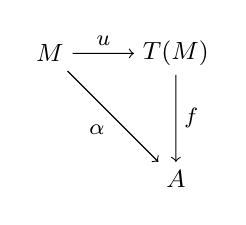
\begin{tikzpicture}[scale=1.6]
            \small
            \node (R) at (0,1) {$M$};
            \node (A) at (1,1) {$T(M)$};
            \node (B) at (1,0) {$A$};
    
            \footnotesize
            \draw [->] (R) -- node[above]     {$u$}      (A);
            \draw [->] (A) -- node[right]     {$f$}      (B);
            \draw [->] (R) -- node[below left]{$\alpha$} (B);
        \end{tikzpicture}
        \caption{Universal property of $T(M)$.}
        \label{fig:univPropTM}
    \end{figure}
    \item Example: We now work out one specific case.
    \item Let's construct $T(M)$ when $M$ is a free $R$-module with $S$ as the basis.
    \begin{itemize}
        \item We have
        \begin{equation*}
            M = \left\{ \sum_{s\in S}c_se_s:c_s\in R,\ S\text{ is finite} \right\}
        \end{equation*}
        \item There's only finitely many nonzero $s$??
        \item If $S$ is finite, then $M=R^S$??
        \item Let $\alpha:M\to A$ with $M$ as above.
        \item To specify $\alpha$, you need only specify its action on a basis of $M$; thus, there is a bijection between the collection of all $\alpha$ and the set $S$ (??) given by $j$??
        \item This induces a ring homomorphism $h:F_R(S)\to A$ given by $h(X_s)=a_s$.
        \item Here, $T(M)=F_R(S)$.
        \item How do you know it doesn't depend on the basis chosen? By the universal property (is this what he said??).
        \item Any module is the quotient of a free module.
    \end{itemize}
    \item There will be more questions on the final like questions 1-2 on the midterm!!!
    \item Certain zeroes exist in $F_R(S)$.
    \item We now start on Section 10.4 and exterior algebras.
    \item $F_R(S)/\gen{X_sX_t-X_tX_s:s,t\in S}$ is the two-sided ideal generated by the given elements. It is the usual/commutative polynomial ring in the $X_s$ ($s\in S$)??
    \item We now move on to the Grassmann algebra.
    \item In calculus, we get things like $v\wedge v=0$ and $v_1\wedge v_2=-v_2\wedge v_1$.
    \item $M$ will always be a free $R$-module on the set $S$ (i.e., with basis $S$) for us.
    \item We now define the \textbf{exterior algebra} of $M$.
    \item \textbf{Exterior algebra} (of $M$): A pair $(A,\alpha)$ where $A$ is an $R$-algebra and $\alpha:M\to A$ is an $R$-module homomorphism such that for all $m\in M$, $\alpha(m)^2=0$. \emph{Denoted by} $\bm{\lam{M}}$.
    \begin{itemize}
        \item We can prove the existence and uniqueness of $\lam{M}$.
    \end{itemize}
    \item Conditions (is this the universal property??).
    \begin{enumerate}
        \item Condition (*) holds for the horizontal arrow, i.e., for $\lam{M}$, $u(m)^2=0$ for all $m\in M$.
        \item If (*) holds for $(A,\alpha)$, then there exists a unique $h$ such that the diagram below commutes.
    \end{enumerate}
    \begin{figure}[H]
        \centering
        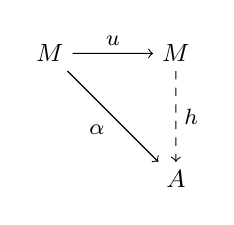
\begin{tikzpicture}[scale=1.6]
            \small
            \node (R) at (0,1) {$M$};
            \node (A) at (1,1) {$\lam{M}$};
            \node (B) at (1,0) {$A$};
    
            \footnotesize
            \draw [->]        (R) -- node[above]     {$u$}      (A);
            \draw [->,dashed] (A) -- node[right]     {$h$}      (B);
            \draw [->]        (R) -- node[below left]{$\alpha$} (B);
        \end{tikzpicture}
        \caption{Existence and uniqueness of the exterior algebra.}
        \label{fig:existUniqueExAlg}
    \end{figure}
    \item $h$ is an $R$-algebra homomorphism such that $(h\circ u)(m)=\alpha(m)$ for all $m\in M$.
    \item Rather than write out the proof, just ask, "why not take $F_R(S)=\lam{M}$?"
    \begin{figure}[H]
        \centering
        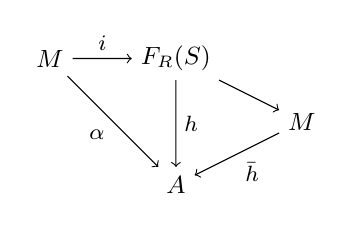
\begin{tikzpicture}[scale=1.6]
            \small
            \node (M) at (0,1)   {$M$};
            \node (F) at (1,1)   {$F_R(S)$};
            \node (A) at (1,0)   {$A$};
            \node (E) at (2,0.5) {$\lam{M}$};
    
            \footnotesize
            \draw [->] (M) -- node[above]      {$i$}       (F);
            \draw [->] (F) -- node[right]      {$h$}       (A);
            \draw [->] (M) -- node[below left] {$\alpha$}  (A);
            \draw [->] (F) --                              (E);
            \draw [->] (E) -- node[below right]{$\bar{h}$} (A);
        \end{tikzpicture}
        \caption{The free $R$-algebra on the set $S$ and the exterior algebra.}
        \label{fig:FRSexAlg}
    \end{figure}
    \begin{itemize}
        \item Consider the above commutative diagram.
        \item Then replace $F_R(S)$ by $F_R(S)/\gen{i(m)^2:m\in M}=\lam{M}$ and extend the commutative diagram.
    \end{itemize}
    \item Let $m=\sum_{s\in S}c_se_s\mapsto\sum_{s\in S}c_sX_s$. We have
    \begin{equation*}
        \left( \sum_sc_sX_s \right)^2 = \sum_{s\in S}c_s^2X_s^2+\sum_{\substack{\{s,t\}\\s\neq t}}c_sc_t(X_sX_t+X_tX_2)
    \end{equation*}
    \item For the moment, the $R$-module spanned modules $X_s^2$ for all $s\in S$, including $X_sX_t+X_tX_s$ and $(X_s+X_t)^2=X_s^2+X_t^2+(X_sX_t+X_tX_s)$.
    \item Something on the difference between $v^2=0$ and $v_1v_2=-v_2v_1$ in normal calculus and what we've done today...??
\end{itemize}



\section{Office Hours (Callum)}
\begin{itemize}
    \item Lecture 7.3: Why did you use the direct product instead of the direct sum in your proof of the RCF theorem? Also, do we still need the $N$ condition on the $m_{i,j}$, or did the way I phrase it suffice? How do you know that there's only finitely many distinct primes?
    \begin{itemize}
        \item If you have a finitely generated PID $R$ and an $R$-module $M$, then is any submodule of $M$ finitely generated?
    \end{itemize}
    \item Problem 7.3?
    \begin{itemize}
        \item It is a straight-up ring problem; we shouldn't be doing anything fancy with modules.
    \end{itemize}
\end{itemize}



\section{Office Hours (Nori)}
\begin{itemize}
    \item \marginnote{2/23:}Lecture 6.1: Proposition proof?
    \item Lecture 6.1: $(2)\subsetneq\Z$ example?
    \item Lecture 6.1: The end of the theorem proof.
    \item Lecture 6.2: Does the first theorem you proved not appear in the book until Chapter 12?
    \item Lecture 6.2: What is $A$ in the proof?
    \item Resources for the proofs in Week 6?
    \item Lecture 7.1: Quotient stuff.
    \item Is my proof for Q7.1(ii) sufficiently not hand-wavey?
    \item Question 7.7?
    \begin{itemize}
        \item Note: The four given submodules satisfy the $T(N)\subset N$ condition even if $M$ does not have the particular form given! It just so happens that in this case, these four are the only allowable ones.
    \end{itemize}
    \item Solving Question 7.7?
    \begin{itemize}
        \item WTS: $N=pM$ or $\ker(p_M)$.
        \item We know that
        \begin{align*}
            pM &= pR/(p^2)\oplus 0&
            \ker(p_M) &= pR/(p^2)\oplus R/(p)
        \end{align*}
        \item $\ker(p_M)$ is a 2D vector space over $R/(p)$.
        \item WTS: $N\cap\ker(p_M)\neq 0$ iff $N\neq 0$.
        \begin{itemize}
            \item We know that $pN\subset N$ by the definition of $N$ as a submodule.
            \item Let $n\in N$ be nonzero. Suppose $n\notin\ker(p_M)$. Then $pn\in\ker(p_M)$. We know that $pn\in N$ as well. Thus, $pn\in N\cap\ker(p_M)$.
        \end{itemize}
        \item $N\cap\ker(p_M)\subset\ker(p_M)$. Thus, $N\cap\ker(p_M)$ is either a 1D or a 2D vector space over $R/(p)$. We WTS that if it's 2D, then it equals $\ker(p_M)$, and if it's 1D, then it equals $pM$.
        \item 2D case.
        \begin{itemize}
            \item We know that $N\cap\ker(p_M)\subset\ker(p_M)$.
            \item 2D implies that $N\not\subsetneq\ker(p_M)$.
            \item Thus, either $N=\ker(p_M)$ or $N\supsetneq\ker(p_M)$.
            \item In the first case, we are done.
            \item In the second case, we can show that this implies that $N=M$.
        \end{itemize}
        \item 1D case.
        \begin{itemize}
            \item We know that $pM\cap\ker(p_M)=p_M$.
            \item Assume $N\neq pM$.
            \item Then $N\cap\ker(p_M)=\gen{(pa,1)}$.
            \item But $T$ exists, where $T:M\to M$ sends $T(1,0)=(1,0)$ and $T(0,1)=(p,1)$.
            \item Therefore we must have $N\cap\ker(p_M)=pM$.
        \end{itemize}
        \item Suppose that $N\supsetneq pM$.
        \begin{itemize}
            \item $N/pM\subset M/pM$. Then use $T(1,0)=(1,1)$ and $T(0,1)=(0,1)$.
        \end{itemize}
    \end{itemize}
\end{itemize}



\section{Exterior Algebra and Determinants}
\begin{itemize}
    \item \marginnote{2/24:}Last time, we were defining the exterior algebra.
    \item Recall:
    \begin{itemize}
        \item We have shown that $\lam{M}$, where $M$ is a free $R$-module with $S$ as basis, equals $F_R(S)/I$.
        \item $F_R(S)$ is a noncommutative polynomial ring in variables $X_s$, with $s\in S$ as variables.
        \item $I$ is the two-sided ideal generated by everything $m^2$ for all $m\in M$ (e.g., $(\sum_{s\in S}c_sX_s)^2$).
        \begin{itemize}
            \item This is also the two-sided ideal generated by $X_s^2$ for all $s\in S$ and $X_sX_t+X_tX_s$ for all $t,s\in S$ with $t\neq s$.
            \item Note that we don't need the $t\neq s$ condition; it just helps to not repeat things.
        \end{itemize}
    \end{itemize}
    \item In $F_R(S)/I$, we have $\overline{X_s^2}=0$ and $X_sX_t=-X_tX_s$. Over real numbers, this is differential forms.
    \item To stop things from repeating, we take a linear ordering of $S$.
    \begin{itemize}
        \item Assume $S=\{1,\dots,n\}$ for simplicity of notation.
        \item We will not have repeated elements in a product, and we can assume that everything comes in linear order.
        \item Let $X_I=X_{i_1}\cdots X_{i_k}$ for $1\leq i_1<\cdots<i_k\leq n$. $I\in\mathcal{P}(\{1,\dots,n\})$.
        \item Thus, we see that the $X_I$, for all $I\in\mathcal{P}(\{1,\dots,n\})$, generates $F_R(S)/I$ as an $R$-module.
        \item We would like to prove this, but Nori will not for time's sake.
    \end{itemize}
    \item We want to show that the $X_I$ are, in fact, a basis.
    \item First approach: Suppose $M=Re_1\oplus\cdots\oplus Re_n$.
    \begin{itemize}
        \item Then let $\mathcal{A}$ be the free $R$-module with $e_I=e_{i_1}\cdots e_{i_k}$ as basis, where $I=\{i_1,\dots,i_k\}$ is in ascending order.
        \item Note: We could put the wedge in all of these products as in calculus, but we can equally well omit it.
        \item If $I\cap J\neq\emptyset$, then $e_Ie_J=0$.
        \item If $I\cap J=\emptyset$, then $e_Ie_J=\sgn(\sigma)e_{I\cup J}$.
        \begin{itemize}
            \item $\sigma$ is the permutation that puts it into ascending order.
        \end{itemize}
        \item Extend multiplication in an $R$-linear way and check that $\mathcal{A}$ is actually a ring. This can be proven via
        \begin{figure}[h!]
            \centering
            
            \caption{Proving that sets with related structure are isomorphic to $F_R(S)/I$.}
            \label{fig:FRSrelated}
        \end{figure}
        \item Then $\lam{Re_1\oplus\cdots\oplus Re_n}$ is a free $R$-module with the $e_I$ as basis.
    \end{itemize}
    \item Second approach: Induction.
    \begin{itemize}
        \item Let $M=Re_1\oplus Re_2\oplus\cdots\oplus Re_n$.
        \item We assume that we have already proven the case $N=Re_2\oplus\cdots\oplus Re_n$.
        \item Let $\lam{N}=A$ be an $R$-algebra.
        \item We wish to construct $B=A\oplus eA$.
        \item Let $\sigma:A\to A$ be defined by $\sigma(n)=-n$ for all $n\in N$. Then $\sigma$ is a ring homomorphism and $\sigma^2(a)=a$.
        \item It follows that $ea=\sigma(a)e$.
        \item We have that
        \begin{equation*}
            (a+be)(c+de) = ac+(ad+b\sigma(c))e
        \end{equation*}
        and this is the ring structure.
        \item Problem: Show that $B$ is a ring when $\sigma:A\to A$ is a ring homomorphism satisfying $\sigma^2=\id$.
    \end{itemize}
    \item We have that $\lam{M}=\bigoplus_{k\geq 0}\lam[k]{M}$.
    \begin{itemize}
        \item Thus, $\rank(M)=n$ where $\lam[k]{M}=0$ for all $k>n$.
    \end{itemize}
    \item Corollary of the universal property: Given $L:M\to N$ an $R$-module homomorphism, then there is a unique $R$-algebra homomorphism called $\lam{L}$ such that the following diagram commutes.
    \emph{picture}
    \item What does $\lam[k]{M}$ mean?
    \begin{itemize}
        \item It is an $R$-module spanned by $e_I$, where the cardinality of $I$ is $k$. This is a bad definition, though.
        \item Better: $R$-submodule of $\lam{R}$ generated by $v_1,\dots,v_k$ where all $v_i\in M$.
    \end{itemize}
    \item Let $\lam{M}=\bigoplus_{k\geq 0}\lam[k]{M}$. Given $L:M\to N$, we get $R$-module homomorphisms called $\lam[k]{L}:\lam[k]{M}\to\lam[k]{N}$ and $\lam{L}(\alpha_0+\alpha_1+\cdots)=\alpha_0+L(\alpha_1)+\lam[2]{L}(\alpha_2)+\cdots$.
    \item Now assume that $\rank(M)=\rank(N)=n$ and $L:M\to N$ is an $R$-module homomorphism. Then $\lam[n]{L}:\lam[n]{M}\to\lam[n]{N}$. This is also called the determinant of $L$.
    \item Now assume that $M=N$. We have a map from a space to itself?? Suppose $\omega$ is a basis element of $\lam[n]{M}$. Then $\lam[n]{L}\omega=\alpha\omega$. There exists such an $\alpha\in R$.
    \begin{itemize}
        \item Then $\lam[n]{L}(a\omega)=a\alpha\omega=\alpha(a\omega)$ for all $a\in R$ and $\lam[n]{L}\eta=\alpha\eta$ for all $\eta\in\lam[n]{M}$.
        \item Let $\det(L)\in R$. Then $\lam[n]{L}\eta=(\det(L))\eta$ for all $\eta\in\lam[n]{M}$.
    \end{itemize}
    \item On the formula for the inverse in terms of adjoint matrices.
    \begin{itemize}
        \item We have $\lam[n-1]{L}:\lam[n-1]{M}\to\lam[n-1]{M}$.
    \end{itemize}
    \item Characteristic polynomial: $M$ is an $R$-module.
    \begin{itemize}
        \item We have $R[\lambda]$ as the polynomial ring in one variable.
        \item $M[\lambda]=M\oplus M\oplus\cdots$ implies that $(m_0,m_1,\dots)$ is $m_0+m_1\lambda+m_2\lambda^2+\cdots$ is an $R[\lambda]$-module.
        \item Let $L:M\to N$ be an $R$-module. Then $L_e:M[\lambda]\to N[\lambda]$ is an $R[\lambda]$-module homomorphism.
        \item Take $M=N$ to be a free $R$-module of rank $n$.
        \item Then $\sum_im_i\lambda^n$ maps to $\sum_iL(m_i)\lambda^i$.
        \item It follows that $M[\lambda]$ and $R[\lambda]$...
        \item We have $\lambda:M[\lambda]\to M[\lambda]$ and $\lambda(m\lambda^i)=m\lambda^{i+1}$. Take $\det(\lambda-L_e)=\det_L(\lambda)\in R[\lambda]$ a monic polynomial of degree $n$.
        \item Then $\lambda^n-\trace(L)\lambda^{n-1}+\cdots+(-1)^n\deg(L)$.
    \end{itemize}
    \item We have $R[\lambda]$ and $\End_R(M)$. Send $\lambda\mapsto L$. This is evaluation at $L$. We also send $c\mapsto c$ for all $c\in R$.
    \item Cayley-Hamilton theorem: $L:M\to M$ is an $R$-module homomorphism and $L$ is free of rank $n$ implies that $\det_L(L)=0$.
    \item We'll get an eighth week summary next Monday.
    \item Next week: A bit of number theory and a bit of geometry. It's up to us whether we come or not. Nori just wants to enjoy himself. None of the content will be on the exam.
\end{itemize}



\section{Chapter 10: Introduction to Module Theory}
\emph{From \textcite{bib:DummitFoote}.}
\setcounter{bookch}{10}
\setcounter{proposition}{7}
\subsection*{Section 10.4: Tensor Products of Modules}
\begin{itemize}
    \item \marginnote{2/26:}Goal: Study the \textbf{tensor product} of two modules over a (not necessarily commutative) ring.
    \item What is the tensor product?
    \begin{itemize}
        \item The construction of a module $M\otimes N$ in which we can take the "product" $mn$ of elements $m\in M$ and $n\in N$.
    \end{itemize}
    \item The general construction is quite complex, so we start with a special case: Extending scalars/changing base.
    \item \textbf{Extension} (of a ring): A ring $S$ related to the original ring $R$ via a ring homomorphism $f:R\to S$ and with the special property that any module on which $R$ acts is acted upon by $f(R)$.
    \item \textbf{Restriction of scalars}: The $R$-module $N$ constructed from the $S$-module $N$ by defining the ring action from $f(R)$ onto $N$, where $f:R\to S$.
    \item Thus, it is possible in general to restrict an $S$-module to an $R$-module.
    \item However, it is \emph{impossible} in general to do the opposite, that is, to extend an $R$-module to an $S$-module.
    \item Examples.
    \begin{itemize}
        \item $\Z$ is a $\Z$-module, but not a $\Q$-module.
        \begin{itemize}
            \item Suppose (contradiction): $\Z$ is a $\Q$-module. Consider the element $z=1/2\cdot 1\in\Z$. Then since
            \begin{equation*}
                1 = 1\cdot 1
                = \left( \frac{1}{2}+\frac{1}{2} \right)\cdot 1
                = \frac{1}{2}\cdot 1+\frac{1}{2}\cdot 1
                = z+z
                = 2z
            \end{equation*}
            there is a $z\in\Z$ such that $2z=1$. But by definition, no such element exists, a contradiction.
        \end{itemize}
        \item However, $\Z\hookrightarrow\Q$.
        \item \textcite{bib:DummitFoote} similarly proves that the $\Z$-module $\Z/2\Z$ cannot be embedded into any $\Q$-module.
    \end{itemize}
    \item \textbf{Embedding}: A natural injection.
    \begin{itemize}
        \item For example, $\Z\hookrightarrow\Q$ is an embedding.
    \end{itemize}
    \item We now construct (for a general $R$-module $N$) the $S$-module that is the "best possible" target in which to try to embed $N$.
    \begin{itemize}
        \item Said module determines \emph{all} possible $R$-module homomorphisms of $N$ into $S$-modules.
        \item In particular, it determines when $N$ is contained in an $S$-module (see Corollary \ref{cly:10.9}).
        \item Example: As per the above, this construction will give us $\Q$ when $R=\Z$ and $S=\Q$.
    \end{itemize}
    \item \textbf{Tensor product} (of $S$ and $N$ over $R$): The quotient group formed from the free $\Z$-module $S\times N$ (a free abelian group) and its subgroup $H$ generated by all elements of the form
    \begin{align*}
        (s_1+s_2,n)-(s_1,n)-(s_2,n)&&
        (s,n_1+n_2)-(s,n_1)-(s,n_2)&&
        (sr,n)-(s,rn)
    \end{align*}
    for $s,s_1,s_2\in S$, $n,n_2,n_2\in N$, and $r\in R$, where $rn$ in the rightmost element above refers to the $R$-module structure already defined on $N$. \emph{Denoted by} $\bm{S\otimes_RN}$, $\bm{S\otimes N}$.
    \begin{itemize}
        \item "Free $\Z$-module $S\times N$:" We mean the collection of all finite commuting sums of elements of the form $(s_i,n_i)$, where $s_i\in S$ and $n_i\in N$.
        \item We denote the coset containing $(s,n)$ in $S\otimes_RN$ by $s\otimes n$.
    \end{itemize}
    \item The quotient definition forces the relations
    \begin{align*}
        (s_1+s_2)\otimes n &= s\otimes n+s_2\otimes n&
        s\otimes(n_1+n_2) &= s\otimes n_1+s\otimes n_2&
        sr\otimes n &= s\otimes rn
    \end{align*}
    \item \textbf{Tensor}: An element of $S\otimes_RN$.
    \begin{itemize}
        \item "Tensors can be written (non-uniquely in general) as finite sums of 'simple tensors' of the form $s\otimes n$ with $s\in S$, $n\in N$" \parencite[360]{bib:DummitFoote}.
    \end{itemize}
    \item The tensor product $S\otimes_RN$ is naturally a left $S$-module under the action defined by
    \begin{equation*}
        s\left( \sum_\text{finite}s_i\otimes n_i \right) = \sum_\text{finite}(ss_i)\otimes n_i
    \end{equation*}
    \begin{itemize}
        \item \textcite{bib:DummitFoote} proves that this expression is well-defined.
        \item \textcite{bib:DummitFoote} performs a rote axiom check.
    \end{itemize}
    \item \textbf{Left $\bm{S}$-module obtained by extension of scalars from the left $R$-module $\bm{N}$}: The module $S\otimes_RN$.
    \item There is a natural map $\iota:N\to S\otimes_RN$ defined by $n\mapsto 1\otimes n$.
    \begin{itemize}
        \item $\iota$ is an $R$-module homomorphism: $1\otimes rn=r\otimes n=r(1\otimes n)$.
        \item $\iota$ is \emph{not} injective in general: Since we pass to a quotient group.
    \end{itemize}
    \item Since $\iota$ need not be injective, we have constructed a natural relation between $N$ and $S\otimes_RN$ but we have not asserted that $S\otimes_RN$ contain an isomorphic copy of $N$.
    \begin{itemize}
        \item In the domain of homomorphisms, though, the fact that the relations we used to construct $H$ and hence $S\otimes_RN$ were the \emph{minimal} ones needed for $S\otimes_RN$ to be a module at all, it is save to assume that $S\otimes_RN$ is the "best possible" $S$-module to serve as the target for an $R$-module homomorphism from $N$.
        \item More precisely, we know this is the best possible one because any other $R$-module homomorphism from $N$ factors through this one. In other words, $\Phi$ below contains all information given by $\varphi$.
    \end{itemize}
    \item What is described above is the \textbf{universal property} (for the tensor product), stated as follows.
    \begin{theorem}\label{trm:10.8}
        Let $R$ be a subring of $S$, let $N$ be a left $R$-module, and let $\iota:N\to S\otimes_RN$ be the $R$-module homomorphism defined by $\iota(n)=1\otimes n$. Suppose that $L$ is any left $S$-module (hence also an $R$-module) and that $\varphi:N\to L$ is an $R$-module homomorphism from $N$ to $L$. Then there is a unique $S$-module homomorphism $\Phi:S\otimes_RN\to L$ such that $\varphi$ factors through $\Phi$, i.e., $\varphi=\Phi\circ\iota$ and the following diagram commutes.
        \begin{figure}[h!]
            \centering
            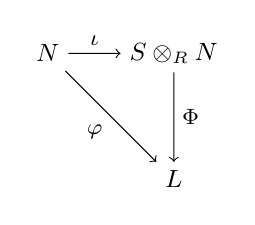
\begin{tikzpicture}[scale=1.6]
                \small
                \node (R) at (0,1) {$N$};
                \node (A) at (1,1) {$S\otimes_RN$};
                \node (B) at (1,0) {$L$};
        
                \footnotesize
                \draw [->] (R) -- node[above]     {$\iota$}   (A);
                \draw [->] (A) -- node[right]     {$\Phi$}    (B);
                \draw [->] (R) -- node[below left]{$\varphi$} (B);
            \end{tikzpicture}
            \caption{Universal property of the tensor product.}
            \label{fig:univPropSotimesRN}
        \end{figure}
        Conversely, if $\Phi:S\otimes_RN\to L$ is an $S$-module homomorphism, then $\varphi=\Phi\circ\iota$ is an $R$-module homomorphism from $N$ to $L$.
        \begin{proof}
            Given.
        \end{proof}
    \end{theorem}
    \item Conditions on when it is possible to map $N$ injectively into some $S$-module, i.e., when some $S$-module contains an isomorphic copy of $N$.
    \begin{corollary}\label{cly:10.9}
        Let $\iota:N\to S\otimes_RN$ be the $R$-module homomorphism in Theorem \ref{trm:10.8}. Then $N/\ker\iota$ is the unique largest quotient of $N$ that can be embedded in any $S$-module. In particular, $N$ can be embedded as an $R$-submodule of some left $S$-module if and only if $\iota$ is injective (in which case $N$ is isomorphic to the $R$-submodule $\iota(N)$ of the $S$-module $S\otimes_RN$).
        \begin{proof}
            Given.
        \end{proof}
    \end{corollary}
    \item Examples.
    \begin{enumerate}
        \item $R\otimes_RN\cong N$.
        \begin{itemize}
            \item Takeaway: Extending scalars from $R$ to $R$ does not change the module.
            \item Proof: Take $\varphi=\id:N\to N$ and $S=R$ in Theorem \ref{trm:10.8}; then $\iota=\Phi^{-1}$ are isomorphisms.
            \item Particular example: If $A$ is any abelian group, then $\Z\otimes_\Z A\cong A$.
        \end{itemize}
        \item More on the $\Z,\Q$ example from above.
        \item Extension of scalars for free modules.
        \item Extension of scalars for vector spaces.
        \item Induced modules for finite groups.
    \end{enumerate}
    \item Return to examples 2-5 later.
    \item We now explore the general tensor product construction, i.e, module 1 need not be a ring $S\supset R$.
    \item First: Two observations about the previous construction.
    \begin{enumerate}
        \item The construction of $S\otimes_RN$ as an abelian group (i.e., before we put the module structure on it) only required quotienting out the elements given in the definition. This quotienting, in turn, only required $S$ to be a \emph{right} $R$-module and $N$ to be a left $R$-module.
        \begin{itemize}
            \item In a similar way, we shall construct an abelian group $M\otimes_RN$ for any \emph{right} $R$-module $M$ and any \emph{left} $R$-module $N$.
        \end{itemize}
        \item The $S$-module structure on $S\otimes_RN$ required only a \emph{left} $R$-module structure on $S$ and the "compatibility relation"
        \begin{equation*}
            s'(sr) = (s's)r
        \end{equation*}
        for all $s,s'\in S$, $r\in R$ between the left $S$-module structure and the right $R$-module structure on $S$.
        \begin{itemize}
            \item We shall also treat the module structure of $M\otimes_RN$ second.
        \end{itemize}
    \end{enumerate}
    \item \textbf{Tensor product} (of $M$ and $N$ over $R$): The quotient group formed from the free $\Z$-module on the set $M\times N$ divided by the subgroup generated by all elements of the form
    \begin{align*}
        (m_1+m_2,n)-(m_1,n)-(m_2,n)&&
        (m,n_1+n_2)-(m,n_1)-(m,n_2)&&
        (mr,n)-(m,rn)
    \end{align*}
    for $m,m_1,m_2\in M$, $n,n_1,n_2\in N$, and $r\in R$, where $N$ is a left $R$-module and $M$ is a right $R$-module. \emph{Denoted by} $\bm{M\otimes_RN}$, $\bm{M\otimes N}$.
    \item \textbf{Tensor}: An element of $M\otimes_RN$.
    \item \textbf{Simple tensor}: A coset $m\otimes n$ of an element $(m,n)\in M\otimes_RN$.
    \item We have the same module-like relations as above, and statement about non-unique decomposition into simple tensors.
    \item Points of care.
    \begin{itemize}
        \item $m\otimes n=m'\otimes n'$ is possible even if $m\neq m'$ or $n\neq n'$.
        \begin{itemize}
            \item Thus, we must exercise care when referring to elements and defining maps based on $m,n$; such a map is only well-defined if it can be shown to be independent of the particular choice of $m\otimes n$ as a coset representative.
        \end{itemize}
        \item When $M,N,R$ may not be clear from context.
    \end{itemize}
    \item \textbf{$\bm{R}$-balanced} (map): A map $\varphi:M\times N\to L$ satisfying
    \begin{align*}
        \varphi(m_1+m_2,n) &= \varphi(m_1,n)+\varphi(m_2,n)&
        \varphi(m,n_1,n_2) &= \varphi(m,n_1)+\varphi(m,n_2)&
        \varphi(m,rn) &= \varphi(mr,n)
    \end{align*}
    for all $m,m_1,m_2\in M$, $n,n_1,n_2\in N$, and $r\in R$, where $M$ is a right $R$-module, $N$ is a left $R$-module, and $L$ is an additive abelian group. \emph{Also known as} \textbf{middle linear with respect to $\bm{R}$}.
    \begin{itemize}
        \item The prototypical $R$-balanced map is $\iota:M\times N\to M\otimes_RN$ defined by $\iota(m,n)=m\otimes n$. We can check all necessary axioms (\textcite{bib:DummitFoote} do this).
    \end{itemize}
    \item We now prove the more general universal property of the tensor product (with respect to balanced maps).
    \begin{theorem}\label{trm:10.10}
        Suppose $R$ is a ring, $M$ is a right $R$-module, and $N$ is a left $R$-module. Let $M\otimes_RN$ be the tensor product of $M$ and $N$ over $R$, and let $\iota:M\times N\to M\otimes_RN$ be the $R$-balanced map defined above.
        \begin{enumerate}
            \item If $\Phi:M\otimes_RN\to L$ is any group homomorphism from $M\otimes_RN$ to an abelian group $L$, then the composite map $\varphi=\Phi\circ\iota$ is an $R$-balanced map from $M\times N\to L$.
            \item Conversely, suppose $L$ is an abelian group and $\varphi:M\times N\to L$ is any $R$-balanced map. Then there is a unique group homomorphism $\Phi:M\otimes_RN\to L$ such that $\varphi$ factors through $\iota$, i.e., $\varphi=\Phi\circ\iota$ as above.
        \end{enumerate}
        Equivalently, the correspondence $\varphi\leftrightarrow\Phi$ in the commutative diagram
        \begin{figure}[H]
            \centering
            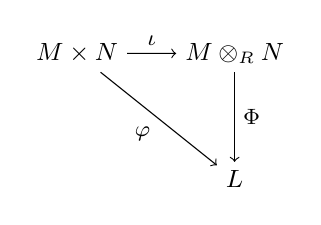
\begin{tikzpicture}[xscale=2,yscale=1.6]
                \small
                \node (R) at (0,1) {$M\times N$};
                \node (A) at (1,1) {$M\otimes_RN$};
                \node (B) at (1,0) {$L$};
        
                \footnotesize
                \draw [->] (R) -- node[above]     {$\iota$}   (A);
                \draw [->] (A) -- node[right]     {$\Phi$}    (B);
                \draw [->] (R) -- node[below left]{$\varphi$} (B);
            \end{tikzpicture}
            \caption{Universal property of the general tensor product.}
            \label{fig:univPropMotimesRN}
        \end{figure}
        establishes a bijection between the $R$-balanced maps $\varphi:M\times N\to L$ and the group homomorphisms $\Phi:M\otimes_RN\to L$.
        \begin{proof}
            Given.
        \end{proof}
    \end{theorem}
    \item Characterizing the tensor product as an abelian group.
    \begin{corollary}\label{cly:10.11}
        Suppose $D$ is an abelian group and $\iota':M\times N\to D$ is an $R$-balanced map such that\dots
        \begin{enumerate}[label={(\roman*)}]
            \item The image of $\iota'$ generates $D$ as an abelian group;
            \item Every $R$-balanced map defined on $M\times N$ factors through $\iota'$ as in Theorem \ref{trm:10.10}.
        \end{enumerate}
        Then there is an isomorphism $f:M\otimes_RN\to D$ of abelian groups with $\iota'=f\circ\iota$.
        \begin{proof}
            Given.
        \end{proof}
    \end{corollary}
    \item We now give $M\otimes_RN$ a module structure.
    \item \textbf{$\bm{(S,R)}$-bimodule}: An abelian group $M$ such that $M$ is a left $S$-module, a right $R$-module, and $s(mr)=(sm)r$ for all $s\in S$, $r\in R$, and $m\in M$, where $R,S$ are rings.
    \item Examples of $(S,R)$-bimodules. Return to later.
    \item \textbf{Standard} ($R$-module structure on $M$): The $(R,R)$-bimodule structure on $M$ defined by letting the left and right $R$-actions coincide, i.e., $mr=rm$ for all $m\in M$ and $r\in R$, where $M$ is a left (or right) $R$ module over the commutative ring $R$.
    \item The tensor product $M\otimes_RN$ is naturally a left $S$-module under the action defined by
    \begin{equation*}
        s\left( \sum_\text{finite}m_i\otimes n_i \right) = \sum_\text{finite}(sm_i)\otimes n_i
    \end{equation*}
    provided that $N$ is a left $R$-module and $M$ is an $(S,R)$-bimodule.
    \begin{itemize}
        \item Proving well-definedness can be done with either analogous calculations to the above, or Theorem \ref{trm:10.10} (return to later).
    \end{itemize}
    \item An important special case of the above general construction: $R$ is commutative and $S=R$.
    \begin{itemize}
        \item This is often the only case considered in works on tensor products!
    \end{itemize}
    \item \textbf{$\bm{R}$-bilinear} (map): A map $\varphi:M\times N\to L$ that is $R$-linear in each factor, that is
    \begin{align*}
        \varphi(r_1m_1+r_2m_2,n) &= r_1\varphi(m_1,n)+r_2\varphi(m_2,n)&
        \varphi(m,r_1n_1+r_2n_2) &= r_1\varphi(m,n_1)+r_2\varphi(m,n_2)
    \end{align*}
    for all $m,m_1,m_2\in M$, $n,n_1,n_2\in N$, and $r\in R$, where $R$ is a commutative ring and $M,N,L$ are $R$-modules. \emph{Also known as} \textbf{2-multilinear}.
    \begin{itemize}
        \item The prototypical $R$-bilinear map is $\iota:M\times N\to M\otimes_RN$, where $M\otimes_RN$ is an $R$-module and $R$ is a commutative ring.
    \end{itemize}
    \item Characterizing $R$-bilinear maps.
    \begin{corollary}\label{cly:10.12}
        Suppose $R$ is a commutative ring. Let $M,N$ be two left $R$-modules and let $M\otimes_RN$ be the tensor product of $M$ and $N$ over $R$, where $M$ is given the standard $R$-module structure. Then $M\otimes_RN$ is a left $R$-module with
        \begin{equation*}
            r(m\otimes n) = (rm)\otimes n
            = (mr)\otimes n
            = m\otimes(rn)
        \end{equation*}
        and the map $\iota:M\times N\to M\otimes_RN$ with $\iota(m,n)=m\otimes n$ is an $R$-bilinear map. If $L$ is any left $R$-module, then there is a bijection between the $R$-bilinear maps $\varphi:M\times N\to L$ and the $R$-module homomorphisms $\Phi:M\otimes_RN\to L$ where the correspondence between $\varphi$ and $\Phi$ is given by the following commutative diagram in Figure \ref{fig:univPropMotimesRN}.
        \begin{proof}
            Given.
        \end{proof}
    \end{corollary}
    \item Examples of tensor products (return to later).
    \item For the rest of the section, we establish some basic properties of the tensor product.
    \item Applying Theorem \ref{trm:10.10} to establish the existence of homomorphisms.
    \begin{theorem}[The "Tensor Product" of Two Homomorphisms]\label{trm:10.13}
        Let $M,M'$ be right $R$-modules, let $N,N'$ be left $R$-modules, and suppose $\varphi:M\to M'$ and $\psi:N\to N'$ are $R$-module homomorphisms.
        \begin{enumerate}
            \item There is a unique group homomorphism $\varphi\otimes\psi:M\otimes_RN\to M'\otimes_RN'$ such that
            \begin{equation*}
                (\varphi\otimes\psi)(m\otimes n) = \varphi(m)\otimes\psi(n)
            \end{equation*}
            for all $m\in M$, $n\in N$.
            \item If $M,M'$ are also $(S,R)$-bimodules for some ring $S$ and $\varphi$ is also an $S$-module homomorphism, then $\varphi\otimes\psi$ is a homomorphism of left $S$-modules. In particular, if $R$ is commutative, then $\varphi\otimes\psi$ is always an $R$-module homomorphism for the standard $R$-module structures.
            \item If $\lambda:M'\to M''$ and $\mu:N'\to N''$ are $R$-module homomorphisms, then
            \begin{equation*}
                (\lambda\otimes\mu)\circ(\varphi\otimes\psi) = (\lambda\circ\varphi)\otimes(\mu\circ\psi)
            \end{equation*}
        \end{enumerate}
        \begin{proof}
            Given.
        \end{proof}
    \end{theorem}
    \item Defining $n$-fold tensor products.
    \begin{theorem}[Associativity of the Tensor Product]\label{trm:10.14}
        Suppose $M$ is a right $R$-module, $N$ is an $(R,T)$-bimodule, and $L$ is a left $T$-module. Then there is a unique isomorphism
        \begin{equation*}
            (M\otimes_RN)\otimes_TL \cong M\otimes_R(N\otimes_TL)
        \end{equation*}
        of abelian groups such that $(m\otimes n)\otimes l\mapsto m\otimes(n\otimes l)$. If $M$ is an $(S,R)$-bimodule, then this is an isomorphism of $S$-modules.
        \begin{proof}
            Given.
        \end{proof}
    \end{theorem}
    \begin{corollary}\label{cly:10.15}
        Suppose $R$ is commutative and $M,N,L$ are $R$-modules. Then
        \begin{equation*}
            (M\otimes N)\otimes L \cong M\otimes(N\otimes L)
        \end{equation*}
        as $R$-modules for the standard $R$-module structures on $M,N,L$.
    \end{corollary}
    \item \textbf{Multilinear} (map): A map $\varphi:M_1\times\cdots\times M_n\to L$ that is an $R$-module homomorphism in each component when the other component entries are kept constant, that is, for each $i\in\{1,\dots,n\}$,
    \begin{equation*}
        \phi(m_1,\dots,rm_i+r'm_i',\dots,m_n) = r\varphi(m_1,\dots,m_i,\dots,m_n)+r'\varphi(m_1,\dots,m_i',\dots,m_n)
    \end{equation*}
    for all $m_i,m_i'\in M_i$ and $r,r'\in R$, where $R$ is a commutative ring and $M_1,\dots,M_n,L$ are $R$-modules under the respective standard $R$-module structures. \emph{Also known as} \textbf{$\bm{n}$-multilinear over $\bm{R}$}.
    \item \textbf{Trilinear} (map): A 3-multilinear map.
    \item The universal property of the tensor product of $n$ modules.
    \begin{corollary}\label{cly:10.16}
        Let $R$ be a commutative ring and let $M_1,\dots,M_n,L$ be $R$-modules. Let $M_1\otimes\cdots\otimes M_n$ denote any bracketing of the tensor product of these modules, and let $\iota:M_1\times\cdots\times M_n\to M_1\otimes\cdots\otimes M_n$ be the map defined by
        \begin{equation*}
            (m_1,\dots,m_n) \mapsto m_1\otimes\cdots\otimes m_n
        \end{equation*}
        Then\dots
        \begin{enumerate}
            \item For every $R$-module homomorphism $\Phi:M_1\otimes\cdots\otimes M_n\to L$, the map $\varphi=\Phi\circ\iota$ is $n$-multilinear from $M_1\times\cdots\times M_n\to L$;
            \item If $\varphi:M_1\times\cdots\times M_n\to L$ is an $n$-multilinear map, then there is a unique $R$-module homomorphism $\Phi:M_1\otimes\cdots\otimes M_n\to L$ such that $\varphi=\Phi\circ\iota$.
        \end{enumerate}
        Hence there is a bijection between the $n$-multilinear maps $\varphi:M_1\times\cdots\times M_n\to L$ and the $R$-module homomorphisms $\Phi:M_1\otimes\cdots\otimes M_n\to L$ with respect to which the following diagram commutes.
        \begin{figure}[H]
            \centering
            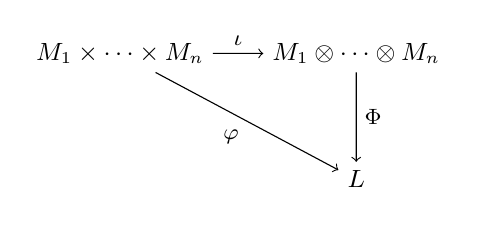
\begin{tikzpicture}[xscale=3,yscale=1.6]
                \small
                \node (R) at (0,1) {$M_1\times\cdots\times M_n$};
                \node (A) at (1,1) {$M_1\otimes\cdots\otimes M_n$};
                \node (B) at (1,0) {$L$};
        
                \footnotesize
                \draw [->] (R) -- node[above]     {$\iota$}   (A);
                \draw [->] (A) -- node[right]     {$\Phi$}    (B);
                \draw [->] (R) -- node[below left]{$\varphi$} (B);
            \end{tikzpicture}
            \caption{Universal property of the $n$-fold tensor product.}
            \label{fig:univPropM1Mn}
        \end{figure}
        \begin{proof}
            We may prove this from first principles analogously to the above. Alternatively, we can invoke Theorem \ref{trm:10.14} and Corollary \ref{cly:10.15} to obtain the $n$-fold tensor product unambiguously and then applying Theorem \ref{trm:10.10} and Corollary \ref{cly:10.12} repeatedly.
        \end{proof}
    \end{corollary}
    \item A sufficient condition for $M_1\subset M$ an $R$-submodule to imply that $M_1\otimes_RN\subset M\otimes_RN$ as an $R$-submodule.
    \begin{theorem}[Tensor Products of Direct Sums]\label{trm:10.17}
        Let $M,M'$ be right $R$-modules and let $N,N'$ be left $R$-modules. Then there are unique group isomorphisms
        \begin{align*}
            (M\oplus M')\otimes_RN &\cong (M\otimes_RN)\oplus(M'\otimes_RN)&
            M\otimes_R(N\oplus N') &\cong (M\otimes_RN)\oplus(M\otimes_RN')
        \end{align*}
        such that $(m,m')\otimes n\mapsto(m\otimes n,m'\otimes n)$ and $m\otimes(n,n')\mapsto(m\otimes n,m\otimes n')$, respectively. If $M,M'$ are also $(S,R)$-bimodules, then these are isomorphisms of left $S$-modules. In particular, if $R$ is commutative, these are isomorphisms of $R$-modules.
        \begin{proof}
            Given.
        \end{proof}
    \end{theorem}
    \item Tensor products commute with direct sums: The generalization of the result; in particular, the statement
    \begin{equation*}
        M\otimes\left( \bigoplus_{i\in I}N_i \right) \cong \bigoplus_{i\in I}(M\otimes N_i)
    \end{equation*}
    \item Applying the above back to the extension of scalars case.
    \begin{corollary}[Extension of Scalars for Free Modules]\label{cly:10.18}
        The module obtained from the free $R$-module $N\cong R^n$ by extension of scalars from $R$ to $S$ is the free $S$-module $S^n$, i.e.,
        \begin{equation*}
            S\otimes_RR^n \cong S^n
        \end{equation*}
        as left $S$-modules.
        \begin{proof}
            Given.
        \end{proof}
    \end{corollary}
    \item The tensor product of two free modules of arbitrary rank over a commutative ring is free. Finite case:
    \begin{corollary}\label{cly:10.19}
        Let $R$ be a commutative ring and let $M\cong R^s$ and $N\cong R^t$ be free $R$-modules with bases $m_1,\dots,m_s$ and $n_1,\dots,n_t$, respectively. Then $M\otimes_RN$ is a free $R$-module of rank $st$ with basis $m_i\otimes n_j$ ($1\leq i\leq s$, $1\leq j\leq t$), i.e.,
        \begin{equation*}
            R^s\otimes_RR^t \cong R^{st}
        \end{equation*}
        \begin{proof}
            Given.
        \end{proof}
    \end{corollary}
    \item Commutativity of the tensor product.
    \begin{proposition}\label{prp:10.20}
        Suppose $R$ is a commutative ring and $M,N$ are left $R$-modules under the standard $R$-module structures. Then there is a unique $R$-module isomorphism
        \begin{equation*}
            M\otimes_RN \cong N\otimes_RM
        \end{equation*}
        mapping $m\otimes n\mapsto n\otimes m$.
        \begin{proof}
            Given.
        \end{proof}
    \end{proposition}
    \item Note that it is not true in general that $M=N$ implies $a\otimes b=b\otimes a$ for all $a,b\in M$.
    \begin{itemize}
        \item Such \textbf{symmetric tensors} are the object of Section 11.6.
    \end{itemize}
    \item The tensor product of $R$-algebras is again an $R$-algebra.
    \begin{proposition}\label{prp:10.21}
        Let $R$ be a commutative ring, and let $A,B$ be $R$-algebras. Then the multiplication $(a\otimes b)(a'\otimes b')=aa'\otimes bb'$ is well-defined and makes $A\otimes_RB$ into an $R$-algebra.
        \begin{proof}
            Given.
        \end{proof}
    \end{proposition}
    \item An example is given to tie a lot of things together.
\end{itemize}



\section{Chapter 12: Modules over Principal Ideal Domains}
\emph{From \textcite{bib:DummitFoote}.}
\setcounter{bookch}{12}
\setcounter{proposition}{11}
\subsection*{Section 12.2: The Rational Canonical Form}
\begin{itemize}
    \item \marginnote{2/21:}As stated previously, we apply the results of Section 12.1 to $F[X]$-modules herein.
    \item Let $V$ be a finite dimensional vector space over $F$ of dimension $N$. Let $(V,T)$ be an $F[X]$-module.
    \item Since $V$ is finite dimensional, it is finitely generated as an $F$-module and hence also as an $F[X]$-module.
    \item If $V$ were free, it would be isomorphic to a direct sum of copies of $F[X]$ (by Theorem \ref{trm:12.5.1}) and hence be infinite dimensional.
    \begin{itemize}
        \item Thus, $V$ is a torsion $F[X]$-module.
        \item Theorem \ref{trm:12.5.3}: $V$ is isomorphic to the direct sum of cyclic, torsion $F[X]$-modules.
        \item This decomposition will allow us to choose a basis for $V$ with respect to which the matrix representation for the linear transformation $T$ is in a specific simple form.
    \end{itemize}
    \item \textbf{Rational canonical form} (of a matrix): The form obtained when we use the invariant factor decomposition of the relevant vector space.
    \item \textbf{Jordan canonical form} (of a matrix): The form obtained when we use the elementary divisor decomposition (and when $F$ contains all the eigenvalues of $T$).
    \item Theorem \ref{trm:12.9} ensures that the RCF and JCF are unique, justifying the labeling of them as \emph{canonical}.
    \item An application of canonical forms: Classifying distinct linear transformations.
    \begin{itemize}
        \item Two matrices that represent the same linear transformation (hence are similar) have the same RCF and JCF.
        \item This is another instance of the structure of the space being acted upon (e.g., the invariant factor decomposition of $V$) providing information on the algebraic objects (e.g., linear transformations) which are acting.
    \end{itemize}
    \item \textbf{Representation Theory of Groups}: The special case of algebraic objects acting on spaces concerning groups acting on vector spaces.
    % \item \textbf{Eigenvalue}: An element $\lambda\in F$ corresponding to a linear transformation $T$ such that there exists a nonzero vector $v\in V$ satisfying $Tv=\lambda v$. \emph{Denoted by} $\bm{\lambda}$.
    % \item \textbf{Eigenvector}: The vector $v$ in the above definition.
    % \item \textbf{Eigenspace} (of a linear transformation corresponding to an eigenvalue): The set of all eigenvectors of a linear transformation $T$ corresponding to a particular eigenvalue $\lambda$ of $T$. \emph{Given by}
    % \begin{equation*}
    %     \{v\in V:Tv=\lambda v\}
    % \end{equation*}
    \item \textbf{Eigenvalues}, \textbf{eigenvectors}, \textbf{eigenspaces}, and the \textbf{determinant} are defined for linear transformations and analogously for matrices.
    \item Properties of eigenvalues.
    \begin{proposition}\label{prp:12.12}
        TFAE.
        \begin{enumerate}
            \item $\lambda$ is an eigenvalue of $T$.
            \item $\lambda I-T$ is a singular linear transformation of $V$.
            \item $\det(\lambda I-T)=0$.
        \end{enumerate}
        \begin{proof}
            Given.
        \end{proof}
    \end{proposition}
    \item \textbf{Characteristic polynomial} (of a linear transformation): The polynomial defined as follows, where $T$ is the linear transformation in question. \emph{Denoted by} $\bm{c_T(X)}$. \emph{Given by}
    \begin{equation*}
        c_T(X) = \det(XI-T)
    \end{equation*}
    % \item \textbf{Characteristic polynomial} (of $A$): The polynomial defined as follows. \emph{Denoted by} $\bm{c_A(X)}$. \emph{Given by}
    % \begin{equation*}
    %     c_A(X) = \det(XI-A)
    % \end{equation*}
    \begin{itemize}
        \item Defined similarly for matrices $A$.
        \item A monic polynomial of degree $\dim V$.
        \item The eigenvalues are the roots.
    \end{itemize}
    \item \textbf{Minimal polynomial} (of of a linear transformation): The unique monic polynomial which generates the ideal $\Ann(V)$ in $F[X]$. \emph{Denoted by} $\bm{m_T(X)}$.
    \begin{itemize}
        \item Defined similarly for matrices $A$.
        \item We know that such a polynomial exists by Theorem \ref{trm:12.5.3}.
        \item Exercise \ref{exr:12.2.5}: The degree of the minimal polynomial is at most $n^2$.
    \end{itemize}
    \item \textbf{Cayley-Hamilton Theorem}: The minimal polynomial for $T$ is a divisor of the characteristic polynomial for $T$.
    \begin{itemize}
        \item Thus, the degree of the minimal polynomial is at most $n$.
    \end{itemize}
    \item We now build up to the \textbf{rational canonical form}.
    \item Introduction.
    \begin{itemize}
        \item Theorem \ref{trm:12.5}: There exists an isomorphism
        \begin{equation}\label{eqn:12.1}
            V \cong F[X]/(a_1(X))\oplus\cdots\oplus F[X]/(a_m(X))
        \end{equation}
        \item The invariant factors $a_i$ are only determined up to units, but since $F[X]^\times=F-\{0\}$, we can make the $a_i$ unique by requiring them to be monic.
        \item Theorem \ref{trm:12.5.3} asserts that $(a_m(X))=\Ann(V)$.
    \end{itemize}
    \item The minimal polynomial and the invariant factors.
    \begin{proposition}\label{prp:12.13}
        The minimal polynomial $m_T(X)$ is the largest invariant factor of $V$. All of the invariant factors of $V$ divide $m_T(X)$.
    \end{proposition}
    \item We now build up to calculating the minimal polynomial of $T$ and the other invariant factors.
    \item Choosing a basis for each of the summands in Equation \ref{eqn:12.1}.
    \begin{itemize}
        \item Recall that the action of $T$ on $V$ is equivalent to the action of $X$ on each summand.
        \item Recall also (from the Example following Proposition \ref{prp:11.1}) that $1,\bar{X},\bar{X}^2,\dots,\bar{X}^{k-1}$ gives a basis of $F[X]/(a(X))$, where $a(X)=X^k+b_{k-1}X^{k-1}+\cdots+b_0$.
        \item With respect to this basis, the linear transformation $T=l_X$ acts via
        \begin{align*}
            1 &\mapsto \bar{X}\\
            \bar{X} &\mapsto \bar{X}^2\\
            \bar{X}^2 &\mapsto \bar{X}^3\\
            &\hspace{2.5mm}\vdots\\
            \bar{X}^{k-2} &\mapsto \bar{X}^{k-1}\\
            \bar{X}^{k-1} &\mapsto \bar{X}^k = -b_0-b_1\bar{X}-\cdots-b_{k-1}\bar{X}^{k-1}
        \end{align*}
        \begin{itemize}
            \item The last equality holds since $a(\bar{X})=0$ in $F[X]/(a(X))$.
        \end{itemize}
        \item With respect to this basis, the matrix for multiplication by $X$ is called the \textbf{companion matrix} of $a(X)$.
        \item Applying this procedure to each of the cyclic modules on the right side of Equation \ref{eqn:12.1} under an appropriate basis yields the \textbf{direct sum} of the companion matrices for the invariant factors as the matrix of $T$.
        \item Note that this matrix is uniquely determined by the invariant factors of the $F[X]$-module $V$. These invariant factors, in turn, uniquely determine $V$ up to isomorphism by Theorem \ref{trm:12.9}.
    \end{itemize}
    \item \textbf{First subdiagonal}: The set of entries in a matrix which lie directly below a diagonal entry. \emph{Also known as} \textbf{subdiagonal}.
    \item \textbf{Companion matrix} (of a polynomial): The $k\times k$ matrix, pertaining to the polynomial $a(X)=X^k+b_{k-1}X^{k-1}+\cdots+b_0$, which consists of 1's down the first subdiagonal, $-b_0,\dots,-b_{k-1}$ down the last column, and zeros elsewhere. \emph{Denoted by} $\bm{\mathcal{C}_{a(X)}}$. \emph{Given by}
    \begin{equation*}
        \mathcal{C}_{a(X)} =
        \begin{pmatrix}
            0      & 0      & \cdots & \cdots & \cdots & -b_0\\
            1      & 0      & \cdots & \cdots & \cdots & -b_1\\
            0      & 1      & \cdots & \cdots & \cdots & -b_2\\
            0      & 0      & \ddots &        &        & \vdots\\
            \vdots & \vdots &        & \ddots &        & \vdots\\
            0      & 0      & \cdots & \cdots & 1      & -b_{k-1}\\
        \end{pmatrix}
    \end{equation*}
    \item \textbf{Direct sum} (of matrices): The block diagonal matrix consisting of the component matrices.
    \begin{itemize}
        \item See the RCF example below.
    \end{itemize}
    \item \textbf{Rational canonical form} (of a matrix): A matrix that is the direct sum of companion matrices for monic polynomials $a_1(X),\dots,a_M(X)$ of degree at least one with $a_1(X)\mid a_2(X)\mid\cdots\mid a_m(X)$. \emph{Also known as} \textbf{RCF}. \emph{Given by}
    \begin{equation*}
        \begin{pmatrix}
            \mathcal{C}_{a_1(X)} &  &  & \\
             & \mathcal{C}_{a_2(X)} &  & \\
             &  & \ddots & \\
             &  &  & \mathcal{C}_{a_m(X)}\\
        \end{pmatrix}
    \end{equation*}
    \item \textbf{Invariant factors} (of the RCF): The polynomials $a_i$ in the above definition.
    \item Definition of a \textbf{block diagonal} matrix.
    \item \textbf{Rational canonical form} (of a linear transformation): The matrix representing $T$ which is in rational canonical form.
    \item \textcite{bib:DummitFoote} proves that the rational canonical form is unique by means of running the generation process in reverse.
    \begin{theorem}[Rational Canonical Form for Linear Transformations]\label{trm:12.14}
        Let $V$ be a finite dimensional vector space over the field $F$, and let $T$ be a linear transformation of $V$.
        \begin{enumerate}
            \item There is a basis for $V$ with respect to which the matrix for $T$ is in rational canonical form, i.e., is a block diagonal matrix whose diagonal blocks are the companion matrices for monic polynomials $a_1(X),\dots,a_m(X)$ of degree at least one with $a_1(X)\mid a_2(X)\mid\cdots\mid a_m(X)$.
            \item The rational canonical from for $T$ is unique.
        \end{enumerate}
    \end{theorem}
    \item Why the \emph{rational} canonical form?
    \begin{itemize}
        \item "Rational" refers to the fact that this canonical form is calculated entirely within the field $F$ and exists for any linear transformation $T$.
        \item This is not the case for the JCF, which only exists if the field $F$ contains the eigenvalues for $T$.
    \end{itemize}
    \item Similar matrices, modules, and the RCF.
    \begin{theorem}\label{trm:12.15}
        Let $S$ and $T$ be linear transformations of $V$. Then TFAE.
        \begin{enumerate}
            \item $S$ and $T$ are similar linear transformations.
            \item The $F[X]$-modules obtained from $V$ via $S$ and via $T$ are isomorphic $F[X]$-modules.
            \item $S$ and $T$ have the same rational canonical form.
        \end{enumerate}
        \begin{proof}
            Given.
        \end{proof}
    \end{theorem}
    \item Observation: Any $n\times n$ matrix $A$ with entries in $F$ arises as the matrix for some linear transformation $T$ of an $n$-dimensional vector space.
    \item This observation allows us to restate Theorems \ref{trm:12.14}-\ref{trm:12.15} in the language of matrices.
    \begin{theorem}[Rational Canonical Form for Matrices]\label{trm:12.16}
        Let $A$ be an $n\times n$ matrix over the field $F$.
        \begin{enumerate}
            \item The matrix $A$ is similar to a matrix in rational canonical form, i.e., there is an invertible $n\times n$ matrix $P$ over $F$ such that $P^{-1}AP$ is a block diagonal matrix whose diagonal blocks are the companion matrices for monic polynomials $a_1(X),\dots,a_m(X)$ of degree at least one with $a_1(X)\mid a_2(X)\mid\cdots\mid a_m(X)$.
            \item The rational canonical from for $A$ is unique.
        \end{enumerate}
    \end{theorem}
    \begin{theorem}\label{trm:12.17}
        Let $A,B$ be $n\times n$ matrices over the field $F$. Then $A,B$ are similar iff $A,B$ have the same RCF.
    \end{theorem}
    \item \textbf{Invariant factors} (of a matrix): The invariant factors of the matrix's RCF.
    \item RCF and similarity questions for $A$ do not depend on which field contains the entries of $A$.
    \begin{corollary}\label{cly:12.18}
        Let $A,B$ be two $n\times n$ matrices over a field $F$, and suppose $F$ is a subfield of the field $K$.
        \begin{enumerate}
            \item The rational canonical form of $A$ is the same whether it is computed over $K$ or over $F$. The minimal and characteristic polynomials and the invariant factors of $A$ are the same whether $A$ is considered as a matrix over $F$ or as a matrix over $K$.
            \item The matrices $A,B$ are similar over $K$ iff they are similar over $F$, i.e., there exists an invertible $n\times n$ matrix $P$ with entries from $K$ such that $B=P^{-1}AP$ iff there exists an (in general different) invertible $n\times n$ matrix $Q$ with entries from $F$ such that $B=Q^{-1}AQ$.
        \end{enumerate}
        \begin{proof}
            Given.
        \end{proof}
    \end{corollary}
    \item Takeaways from Corollary \ref{cly:12.18}.
    \begin{itemize}
        \item The RCF for $A$ is an $n\times n$ matrix with entries in the smallest field containing the entries of $A$.
        \item Further explanation of the word \emph{rational}: The RCF is the same matrix even if we allow conjugation of $A$ by nonsingular matrices whose entries come from larger fields.
    \end{itemize}
    \item Characteristic polynomials and invariant factors.
    \begin{lemma}\label{lem:12.19}
        Let $a(X)\in F[X]$ be any monic polynomial.
        \begin{enumerate}
            \item The characteristic polynomial of the companion matrix of $a(X)$ is $a(X)$.
            \item If $M$ is the block diagonal matrix
            \begin{equation*}
                M =
                \begin{pmatrix}
                    A_1 & 0 & \cdots & 0\\
                    0 & A_2 & \cdots & 0\\
                    \vdots & \vdots & \ddots & \vdots\\
                    0 & 0 & \cdots & A_k\\
                \end{pmatrix}
            \end{equation*}
            given by the direct sum of matrices $A_1,\dots,A_k$, then the characteristic polynomial of $M$ is the product of the characteristic polynomials of $A_1,\dots,A_k$.
        \end{enumerate}
        \begin{proof}
            See the exercises.
        \end{proof}
    \end{lemma}
    \begin{proposition}\label{prp:12.20}
        Let $A$ be an $n\times n$ matrix over the field $F$.
        \begin{enumerate}
            \item The characteristic polynomial of $A$ is the product of all the invariant factors of $A$.
            \item (The Cayley-Hamilton Theorem) The minimal polynomial of $A$ divides the characteristic polynomial of $A$.
            \item The characteristic polynomial of $A$ divides some power of the minimal polynomial of $A$. In particular, these polynomials have the same roots, not counting multiplicities.
        \end{enumerate}
        \begin{proof}
            Given.
        \end{proof}
    \end{proposition}
    \item The relations in Proposition \ref{prp:12.20} are frequently useful in determining the invariant factors of $A$, particularly for $\deg(A)$ small.
    \item \textbf{Elementary row and column operations}: The following three operations, where $A$ is an $n\times n$ matrix over the field $F$ and $XI-A$ is an $n\times n$ matrix with entries in $F[X]$. \emph{Given by}
    \begin{enumerate}[label={(\roman*)}]
        \item Interchanging two rows or columns.
        \item Adding a multiple (in $F[X]$) of one row or column to another.
        \item Multiplying any row or column by a unit in $F[X]$, i.e., by a nonzero element in $F$.
    \end{enumerate}
    \item \textbf{Smith Normal Form} (of a matrix): The following form of the $n\times n$ matrix $XI-A$ with entries from $F[X]$, where $a_1,\dots,a_m$ are the invariant factors of $A$. \emph{Given by}
    \begin{equation*}
        \begin{pmatrix}
            1\\
            & \ddots\\
            && 1\\
            &&& a_1(X)\\
            &&&& a_2(X)\\
            &&&&& \ddots\\
            &&&&&& a_m(X)\\
        \end{pmatrix}
    \end{equation*}
    \item Computing the invariant factors in general.
    \begin{theorem}\label{trm:12.21}
        Let $A$ be an $n\times n$ matrix over the field $F$. Using the three elementary row and column operations above, the $n\times n$ matrix $XI-A$ is with entries in $F[X]$ can be put into Smith Normal Form.
    \end{theorem}
    \item \textcite{bib:DummitFoote} provides algorithms for computing the invariant factor decomposition and the RCF. Return to later.
\end{itemize}

\subsubsection*{Exercises}
\begin{enumerate}[label={\textbf{\arabic*.}},ref={12.2.\arabic*},start=5]
    \item \label{exr:12.2.5}Prove directly from the fact that the collection of all linear transformations of an $n$-dimensional vector space $V$ over $F$ to itself form a vector space over $F$ of dimension $n^2$ that the minimal polynomial of a linear transformation $T$ has degree at most $n^2$.
\end{enumerate}




\end{document}